\section{Appendix}
\subsection{File formats}
Files with extension ``ranks\_sorted''  are the actual trace results.
The fields in the table in this file:
\begin{itemize}
\item {\tt alignment\#}     number of the position in the alignment
\item {\tt residue\#}        residue number in the PDB file
\item {\tt type}            amino acid type
\item {\tt rank}            rank of the position according to older version of ET
\item {\tt variability}     has two subfields:
  \begin{enumerate}
                \item number of different amino acids appearing in
                    in this column  of the alignment
                \item  their type
  \end{enumerate}
		  
\item {\tt rho}             ET score - the smaller this value, the lesser variability
                of this position across the branches of the tree
                (and presumably the greater the importance for the protein)
\item {\tt cvg}             coverage - percentage of the residues on the structure which
                have this rho or smaller
\item {\tt gaps}            percentage of gaps in this column
\end{itemize}

\subsection{Color schemes used}
\begin{figure} [t]
{
  \center
  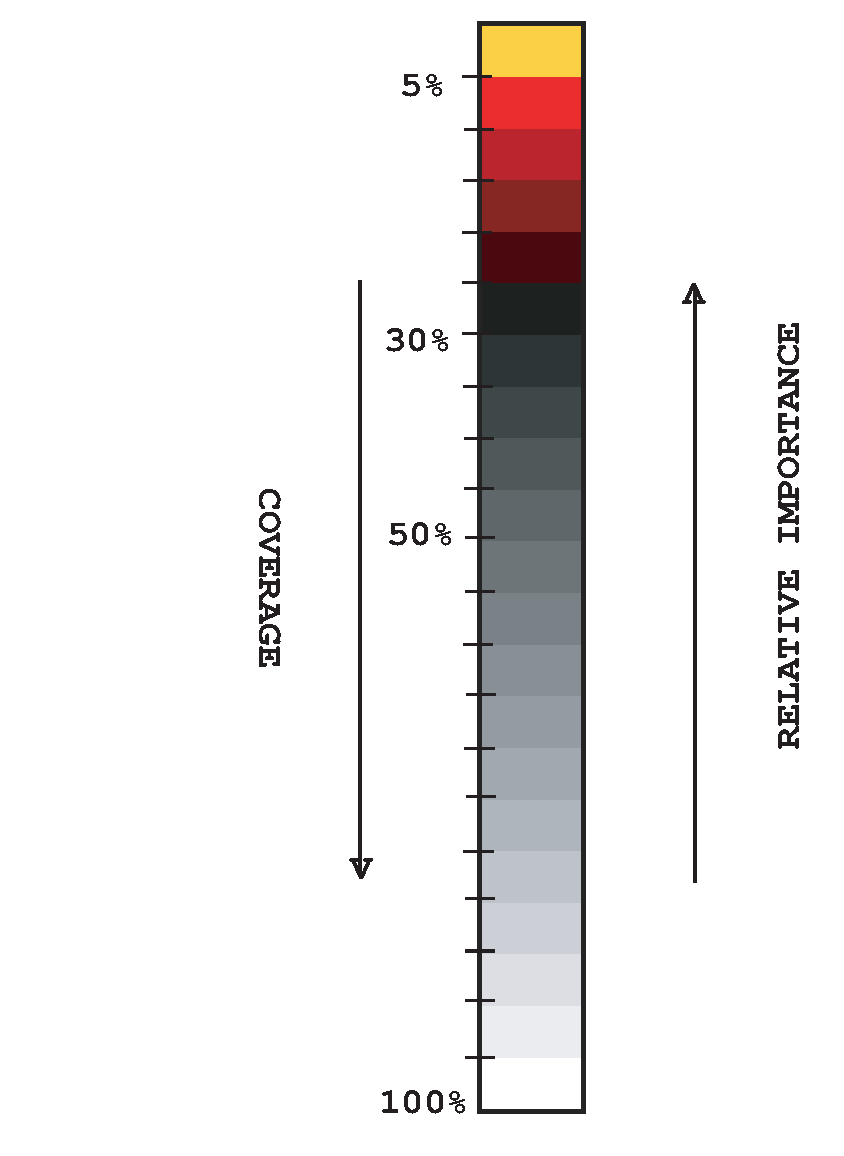
\includegraphics[height=60mm] {colorbar.eps}
}
\caption{\label{colorbar} Coloring scheme used to color residues by their relative importance.}
\end{figure}


The colors used to distinguish the residues by the estimated  evolutionary pressure they experience can
be seen in Fig. \ref{colorbar}.

\subsection{Alistat output}
\emph{alistat} reads a multiple sequence alignment from the file, and shows a number of simple statistics about it. 
These statistics include the name of the format, the number of sequences, 
the total number of residues, the average and range of the sequence lengths, the alignment length (e.g. including gap characters).

Also shown are some percent identities. A percent pairwise alignment identity is defined as (idents / MIN(len1, len2)) 
where idents is the number of exact identities and len1, len2 are the unaligned lengths of the two sequences. 
The "average percent identity", "most related pair", and "most unrelated pair" of the alignment are the average,
 maximum, and minimum of all (N)(N-1)/2 pairs, respectively. 
The "most distant seq" is calculated by finding the maximum pairwise identity 
(best relative) for all N sequences, then finding the minimum of these N numbers (hence, the most outlying sequence). 
\emph{alistat} is copyrighted by  HHMI/Washington University School of Medicine, 1992-2001,
and freely distributed under the GNU General Public License.


\subsection{Citing this work}
The method used to make predictions is this report can be found in 
Mihalek, I., I. Res, O. Lichtarge. (2004).
\emph {"A Family of Evolution-Entropy Hybrid Methods for Ranking of Protein Residues by Importance" }
J. Mol. Bio. {\bf 336}: 1265-82.
For the original version of ET see
O. Lichtarge, H.Bourne and F. Cohen  (1996).
\emph {"An Evolutionary Trace Method Defines Binding Surfaces Common to Protein Families" }
J. Mol. Bio. {\bf 257}: 342-358.
